\documentclass{beamer}
\usepackage[utf8]{inputenc}
\usepackage[french]{babel}
%\usepackage[T1]{fontenc}
\usepackage{graphicx}
%\usepackage{csquotes}

% 20 minutes presentation time

\title{Investigation sur les différences dans les interactions
  enseignant-élèves selon le sexe de l’élève dans les classes
  de physique}
\subtitle{Une étude pilote }
\author{Sofia Vallecorsa \& Paul Maley}
\date{29 juin 2017}

\begin{document}

%% Titlepage
\frame{\titlepage}

%% TOC
\begin{frame}
\frametitle{Table de matières}
\tableofcontents
\end{frame}

%% Introduction
\section{Introduction}
\begin{frame}
\frametitle{Introduction}
\begin{itemize}
\item L'inégalité d'emploi entre hommes et femmes dans les métiers STEM est une évidence.
\item Les origines de cette inégalité (surtout concernant la part joué par la scolarité) sont le sujet de beaucoup d'études.
	\begin{itemize}
	\item Les stéréotypes de genre
	\item Le contexte scolaire, l'approche didactique, mais aussi la transposition didactique
	\item L'attitude des enseignants et leur interactions avec les élèves	
	\end{itemize}		 
\end{itemize}
\end{frame}

%%Introduction -- Les stéréotypes
\begin{frame}
\frametitle{Les stéréotypes de genre}
\begin{itemize}
\item Les modes d’accès à la connaissance sont différents entres filles et garçons à partir du plus jeune âge
\item Les différents rôles sociaux s’imposent très vite dans l’éducation des enfants dans la famille, à l’école et dans tous les aspects de la vie sociale
\item Quand ils arrivent à l'école les jeunes ont souvent déjà interiorisé ces stéréotypes
\item L’école devrait corriger cette tendance et promouvoir une égalité de base entre les sexes
\end{itemize}
\end{frame}

%%Introduction -- Le contexte scolaire
\begin{frame}
\frametitle{Le contexte scolaire}
\begin{itemize}
	\item Selon la vision anthropologique des savoirs (Chevallard, 1985), la construction d’un savoir se fait à l’intérieur d’une institution qui véhicule le rapport élève-savoir
\item Il existe donc l'institution "ecole" et les institutions "extérieures"
\item Les références extérieures à l'école jouent un rôle predominant
\item La question reste ouverte
\end{itemize}
\end{frame}

%%Introduction -- La transposition didactique
\begin{frame}
\frametitle{La transposition didactique}
\begin{itemize}
\item Beaucoup d’études soulignent que les sciences sont présentées dans un contexte masculin (plus attractives pour les garçons)
\item Ex. Les situations d’entrée des séquences d’investigations presentent des personnages masculins dans la vaste majorité (70\%) (Morge & Capelle-Toczek, 2010)
\item Les enseignants sont aussi porteurs (in-)conscients de stéréotypes de sexe
\end{itemize}
\end{frame}

%%Introduction -- L'attitude des enseignants
\begin{frame}
\frametitle{L'attitude des enseignants}
\begin{itemize}
\item La quantité et qualité d’interactions varient  selon le sexe des étudiants (Duru-Bellat, 1994)
\item L'observation des pratiques enseignantes dans des séquences enregistrées dans des classes de mathématiques, montre des différences, quantitatives et qualitatives, de traitement des élèves selon leur sexe (Mosconi, 2001)
\item (Chevet, 2006) Souligne les différences entre les consignes et les explications des tâches données aux filles ou garçons
\item En Suisse, une étude sur l’évaluation dans les cours de physique (Hofer, 2015) montre comment les femmes reçoivent des notes inférieures aux hommes.
\end{itemize}
\end{frame}

%% Problématique
\section{Problématique}
\begin{frame}
\frametitle{Problématique}
\begin{itemize}
\item Notre projet propose d'investiguer une seule cause potentielle parmi beaucoup -- l'interaction entre enseignant et élève.
\end{itemize}
\end{frame}

\begin{frame}
\frametitle{Problématique}
\begin{block}{ }
Y a-t-il une différentiation dans les interactions enseignants-élèves entre les élèves masculins et les élèves féminines dans les écoles secondaires en Suisse Romandes?'
\end{block}
\end{frame}

%% Méthodologie
\section{Méthodologie}
\subsection{Méthodologie standard}
\begin{frame}
\frametitle{Méthodologie standard}
\begin{itemize}
<<<<<<< HEAD
\item La méthodologie ``standarde'' pour chercher une telle différence serait d'enregistrer des séance de classe et d'analyser
les interactions selon un cadre théorique. La théorie des actions conjoints en didactiques (TACD) semble être un bon choix.
=======
\item La méthodologie ``standard'' pour chercher une telle différence serait d'enregistrer des séance de classe et d'analyser
les interactions selon un cadre théorique. La théorie des actions didactiques conjoints (TACD) semble être un bon choix.
>>>>>>> 6ff0e09f4584e99f82ce5bfcb4297facc7c81352
\item Une telle analyse permettrait d'observer des différences mais pour en venir à la raison d'être de ces différences il faudrait articuler ces obsevations avec des entretiens enseignants.
\item Pour comprendre si ces différences sans généralisés ou des cas isolés il en faudra beaucoup de vidéos.
\item Cette approche est limitée par le temps qu'il faut pour analyser des séquences vidéos mais aussi par des questions
légales -- vision des vidéos par autrui.  
\end{itemize}
\end{frame}

\subsection{Notre approche}
\begin{frame}
\frametitle{Notre approche -- le questionnaire}
\begin{itemize}
\item Nous avons imaginé une approche alternative.
\item Utiliser un questionnaire où chaque question propose:
  \begin{itemize}
   \item Une situation et le début d'une transaction didactique en classe
   \item Deux options pour comment poursuivre la transaction 
  \end{itemize}
\item Le questionnaire est presenté aux répondants comme une étude sur
  ``la posture didactique'' de l'enseignant(e).
\item Le répondant est encouragé de visualiser la situation et choisir la
  réponse la plus apte. 
\end{itemize}
\end{frame}

\begin{frame}
\frametitle{Notre approche -- Les biais possibles}
\begin{itemize}
\item Le professeur accepte un niveau de travail plus médiocre chez les filles.
\item Le professeur accorde moins de temps (d’attention) aux filles dans la classe (Spender, 1982)
\item Le professeur s’intéresse davantage aux garçons en échec qu’aux filles.
\item Le professeur laisse plus de temps aux garçons pour répondre aux questions qu’il n’en accorde aux filles.
\item Le professeur croit que les garçons sont plus forts en maths (cela n’est pas du tout subconscient!) (Jusim, 1991).
\item Les problèmes ont plus souvent un contexte masculin.
\end{itemize}
\end{frame}

\begin{frame}
\frametitle{Notre approche -- fonctionnement}
\begin{itemize}
\item Le questionnaire existe en deux version: A/B.
\item Dans chaque question le sexe de l'élève est inversé entre les questionnaires.
\item Un intéraction différencié selon le sexe se manifeste dans une différence
dans la proportion de chaque réponse choisit entre les deux questionnaires (A/B). 
  
\end{itemize}
\end{frame}


\begin{frame}
\frametitle{Notre approche -- Un exemple (Version A)}
\begin{block}{Question – Classe 1M}
Vous demandez à la classe la distance approximative entre la lune et la terre (sujet discuté la veille) et plusieurs élèves (Zoe entre eux) lèvent la main. Vous donnez la parole à Zoe mais elle hésite :
\end{block}

\begin{block}{Réponses}
\begin{itemize}
\item Vous attendez quelques secondes pour sa réponse.
\item Vous passez à quelqu’un d’autre (ça doit être une simple restitution).
\end{itemize}
\end{block}

Version B est pareil avec Zoe remplacé par Nathan.
\end{frame}

\begin{frame}
\frametitle{Notre approche -- la théorie}
\begin{itemize}
\item Les deux manières de poursuivre la transaction sont raisonables.
\item Les enseignants peuvent avoir une préférence pour une où l'autre.
\item La différence entre les deux réponses doit être tel qu'elle serait
  observable dans la classe -- dans l'exemple précédente c'est le temps
  accordé à une élève pour répondre.
\item Cette question simule l'analyse d'une ensemble de vidéos où on
  observe le temps accordé aux élèves pour répondre et en particulier
  pour voir si c'est égal entre garçons et filles.
\end{itemize}
\end{frame}

\begin{frame}
  \frametitle{La théorie des actions cojointe en didatique (TACD)}
  \begin{itemize}
    \item Une théorie avec laquelle un checheur peut analyser des interactions
      dans la classe.
    \item Nous l'avons utiliser pour imaginer comment on peut varier
      les réponse proposées dans chaque question.
      \item Cette élaboration des questions est loin d'être facile.
    \end{itemize}
\end{frame}

\section{Étude pilote}
\begin{frame}
\frametitle{Étude pilote}
  \begin{itemize}
  \item Nous avons mis les deux questionnaires sur SurveyMonkey et envoyé des liens aux étudiant(e)s
  physicien(ne)s de l'HEP.
  \item 7 étudiant(e)s ont rempli les sondages.
    \item 3 version A, 4 version B.
    \end{itemize}

\end{frame}

%% Survey results
\begin{frame}
  \frametitle{Résultats}

  \begin{center}
\hspace*{-1.5cm}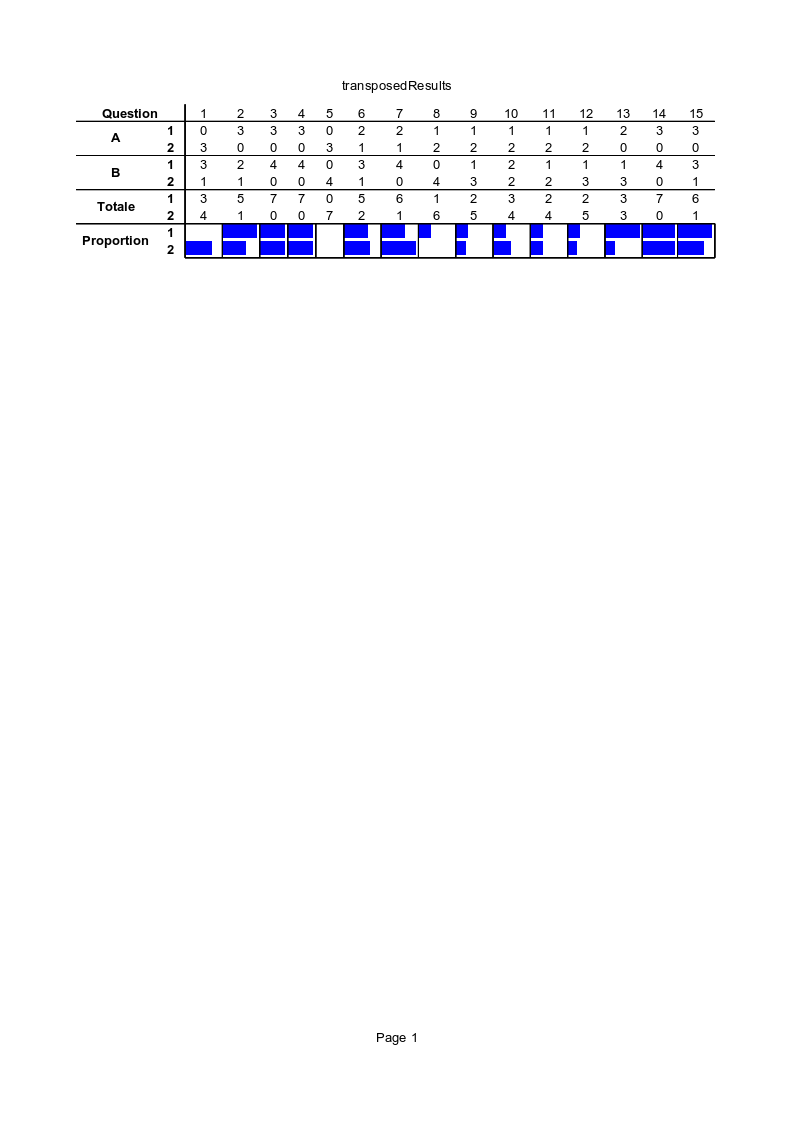
\includegraphics[scale=0.5]{transposedResults}%\hspace*{4cm}
\end{center}
  \end{frame}


%% Analyse
\section{Analyse}
\begin{frame}
  \frametitle{Analyse}
  \begin{itemize}
  \item Peu d'observation -- on s'intéresse à la construction du questionnaire.
  \item 4 questions (3, 4, 5, 14) ont toutes les réponses pareilles -- à refaire
  \item 4 questions (2, 7, 8, 15) ont 6 contre 1 -- à reconsiderer
  \item 7 questions (1, 6, 9, 10, 11, 12, 13) ont des réponses bien partagés
    entre les deux choix -- Questions utiles
  \end{itemize}
\end{frame}

\begin{frame}
  \frametitle{Les ``mauvaises'' questions}
  \begin{itemize}
  \item Tout le monde a choisit la même réponse -- donc on peut imaginer que les deux réponses étaient
  trop écartés une de l'autre et il faut les repenser.
  \item Au même temps nouns nous demandons si'il y a un effet ``ce que je devrais faire'' plutôt que ``ce que 
  je ferais''? Sur tout parce que nous avon essayé de rester proche à nos propres expériences.
 \item Le choix de la réponse a été fait plutôt  pour des raisons pédagogiques  
 \item Questions mal posé ou a reformuler de façon plus "subtile"
%\item Question où une reponse avait une valeur pedgogique beaucoup plus "prononcié" que l'autre
\end{itemize}
\end{frame}

\begin{frame}
  \frametitle{Les ``bonnes'' questions}
  \begin{itemize}
  \item Une répartion assez équilibré entre les deux réponses proposées.
  \item  Des candidats à l'investigation des biais (avec un plus de données disponibles)
  \end{itemize}
\end{frame}

\begin{frame}
  \frametitle{Deux exemples}
  \begin{itemize}
  \item Question 1:
    \begin{enumerate}
    \item Vous renvoyez Samantha lire le protocole. 
    \item Vous accompagnez Samantha à sa place pour regarder le protocole ensemble. 
    \end{enumerate}
  \item Version A (Samantha) 3/3 pour réponse 2.
  \item Version B (Arnaud) 3/4 pour réponse 1.
  \item Inférence: Attente que les garçons se débrouillent mais que les filles ont
    besoin d'aide?\footnote{Pas statistiquement significant} 
  \end{itemize}
\end{frame}

\begin{frame}
  \frametitle{Deux exemples}
  \begin{itemize}
  \item Question 13:
    \begin{enumerate}
    \item «OK, s’ils montent ensemble, ils s’ajoutent; qu’est-ce qui détermine
      s’ils montent ensemble ou pas?
    \item «OK, donc ce que vous décrivez est l’interférence entre deux ondes.
      Quelle est la condition pour que l’interférence soit constructive?»   
      \end{enumerate}
  \item Version A (Laura) 2/2 pour réponse 1.
  \item Version B (Martin) 3/4 pour réponse 2.
  \item Inférence: posture de l'enseignant accompagnant pour les filles,
    analytique pour les garçons?\footnote{Pas statistiquement significant} 
  \end{itemize}
\end{frame}


%% Conclusions
\section{Conclusions}
\subsection{Conclusions de l'étude pilote}
\begin{frame}
\frametitle{Conclusions de l'étude pilote}
  \begin{itemize}
  \item Les résultats nous donne confiance que cette approche pourrait fonctionner.
  \item Nous voyons que certains questions ne sont pas bonnes - tout le monde
    choisit la même réponse. Ces questions devraient être changées pour la suite.
  \end{itemize}
\end{frame}

\subsection{La suite}
\begin{frame}
  \frametitle{La suite}
  \begin{itemize}
  \item Nous pensons que cette approche pourrait être reprise pas quelqu'un(e).
  \item Remplacer ou modifier les questions qui ne sont pas bonnes.
  \item Produire plus de questions.
    \item (?) Utiliser de manière plus explicite la TACD
  \item Analyser aussi en terme du sexe et expérience de l'enseignant(e).
    \item Si des biaises sont observés articuler les résultats avec des entretiens.
  \end{itemize}
\end{frame}

\subsection{Perspectives}
\begin{frame}
  \frametitle{Perspectives}
  \begin{itemize}
  \item Etablir un cadre legale explicite (selon le recommendations du rapport du Centre suisse de coordination pour la recherche en éducation )
  \item Rendre obligatoire pour les enseignants « une formation sur le genre qui puisse expliciter le danger, expliquer les enjeux  et donner des pistes d’intervention pratiques » (Baurens, Schreiber, 2010). 
  \item Etre capables d’analyser leur propre interaction et corriger les façons d’enseigner 
  \item ..et surtout... motiver les élèves!  Les écoles qui sont capables d’attirer le plus d’étudiants sont aussi les écoles où la différence de sexe est  moins évidente". (Erdogan, Stuessy, 2015). 	  
  \end{itemize}
\end{frame}

\section{Annexes}
%% Bibliographie
\begin{frame}
\frametitle{Bibliographie}
\end{frame}

\begin{frame}
  \frametitle{Hypothesis test on $p_A = p_B $}
  \begin{description}
  \item[$H_0$] La proportion des répondants ayant choisi la réponse 1 est
                pareille dans les questionnaires A et B: $p_A = p_B$. 
  \item[$H_A$] La proportion des répondants ayant choisi la réponse
                1 n’est pas  pareille dans les questionnaires A et B: $p_A \ne p_B$.
  \end{description}
  Où $p_{A/B}  = \frac{n_{1A/B}}{n_{1A/B}  + n_{2A/B}}$.

  \[
  Z = \frac{(p_A-p_B) - 0}{\sigma} ,\quad
  \sigma = \sqrt{\frac{p_A(1-p_A)}{n_A} + \frac{p_B(1-p_B)}{n_B}} 
  \]
  Constrainte: $n_{A/B} \cdot p_{A/B} > 5$, $n_{A/B} \cdot (1-p_{A/B}) > 5$ 
\end{frame}

\begin{frame}
  \frametitle{Hypothesis test of $\chi^2$ -- I}
Exemple -- Analyse de Q1:


\begin{center}
\begin{tabular}{c|cc|c}
   & \multicolumn{2}{c|}{Version} &  \\ 
  Réponse  & A & B & Totale \\ \hline
  1 & 0 & 3 & 3 \\
  2 & 3 & 1 & 4 \\ \hline
  Totale & 3 & 4 & 7
\end{tabular}
\end{center}

\begin{description}
\item [$e_{ij}$] Valeur dans le cellule ${ij}$ basé sur indépendence entre
  {\bf version} et {\bf réponse}.
\item [$o_{ij}$] Valeur observé dans le cellule ${ij}$.
\end{description}

par exemple $e_{11} = \frac{3}{7} \cdot \frac{3}{7}$
\end{frame}

\begin{frame}
\frametitle{Hypothesis test of $\chi^2$ -- II}

Calculer le statistique:
\[
\chi^2 = \sum_{ij} \frac{(e_{ij}-o_{ij})^2}{e_{ij}}
\]

  \begin{description}
  \item[$H_0$] Les deux variables sont independentes. 
  \item[$H_A$] Les deux variables ne sont pas independentes.
  \end{description}

  Choisir un niveau de confiance pour obtenir $\chi^2_{\text{critique}}$ et comparer avec
  la valeur de $\chi^2$ calculée (nombre de degrés de liberté: 1). 
\end{frame}


\end{document}
